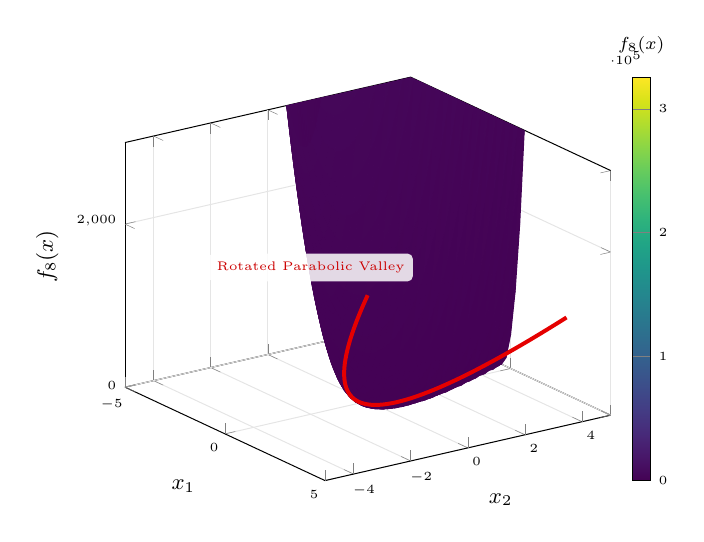
\begin{tikzpicture}[scale=0.9, every node/.style={transform shape}]
\begin{axis}[
    view={55}{25},
    xlabel={$x_1$},
    ylabel={$x_2$},
    zlabel={$f_8(x)$},
    xmin=-5, xmax=5,
    ymin=-5, ymax=5,
    zmin=0, zmax=3000,
    colormap/viridis,
    colorbar,
    colorbar style={title={\scriptsize $f_8(x)$}, width=0.25cm},
    tick label style={font=\tiny},
    label style={font=\small},
    grid=major,
    grid style={gray!20}
]
    % Official BBOB f8 (Instance 1, D=2):
    % Incorporates spatial shift x* and rotation R:
    % z1 = 0.8*x1 + 0.6*x2 - 0.5
    % z2 = -0.6*x1 + 0.8*x2 + 0.2
    % f8 = 100*(z2 - z1^2)^2 + (1 - z1)^2
    \addplot3[
        surf,
        domain=-5:5,
        domain y=-5:5,
        samples=45,
        shader=flat
    ] {
        100 * (( -0.6*\x + 0.8*\y + 0.2 ) - (0.8*\x + 0.6*\y - 0.5)^2 )^2 + (1 - (0.8*\x + 0.6*\y - 0.5))^2
    };

    % Highlighting the Transformed Parabolic Valley Path
    \addplot3[
        red!90!black,
        ultra thick,
        domain=-3:3,
        samples=60,
        samples y=0
    ] (
        { 0.8*x - 0.6*x^2 + 0.28 }, 
        { 0.6*x + 0.8*x^2 - 0.14 }, 
        { (1 - x)^2 }
    );

    % Annotation for the Transformed Minimum / Valley
    \node[fill=white, fill opacity=0.85, text opacity=1, rounded corners=2pt, font=\tiny, text=red!80!black] 
        at (axis cs:0, -2, 1800) {Rotated Parabolic Valley};

\end{axis}
\end{tikzpicture}